%-----------------------------------------------------------------------------%
\chapter{\topikEmpat}
%-----------------------------------------------------------------------------%

%-----------------------------------------------------------------------------%
\section{Pendahuluan}
%-----------------------------------------------------------------------------%

AMBER (\f{Assisted Model Building with Energy Refinement}) adalah paket program untuk menjalankan simulasi dinamika molekular (\f{molecular dynamics}) yang dikembangkan oleh \f{University of California}, San Fransico. Alamat \f{website} resmi dari AMBER adalah \url{http://ambermd.org}.

AMBER digunakan untuk berbagai eksperimen dinamika molekular seperti simulasi pergerakan fisik dari atom dan molekular, pemodelan protein dan eksperimen yang terkait dengan perancangan obat (\f{drug discovery}).

AMBER didistribusikan dalam dua bagian:

\begin{enumerate}
	\item AMBER (berbayar, versi terakhir 14)
	\item AMBERTool (\f{opensource} GPL, versi terakhir 15)
\end{enumerate}

AMBER memiliki dua mode instalasi, yaitu berbasis CPU (dengan OpenMPI) dan berbasis GPU (dengan CUDA). Petunjuk instalasi dapat dilihat di \url{http://jswails.wikidot.com/installing-amber14-and-ambertools14}.

%-----------------------------------------------------------------------------%
\section{Eksperimen}
%-----------------------------------------------------------------------------%

Percobaan dilakukan dengan menjalankan 6 buah eksperimen yang disediakan pada AMBER GPU \f{Benchmark Suite} yang diperoleh dari \f{website} resmi AMBER \url{http://ambermd.org/Amber14_Benchmark_Suite.tar.bz2}. Enam buah eksperimen yang kami jalankan adalah:

\begin{enumerate}
	\item \verb|TRPCAGE Production| (304 atoms, 1.000 nsteps)
	\item \verb|Myoglobin Production| (2,492 atoms, 25.000 nsteps)
	\item \verb|JAC Production NVE| (23,558 atoms, 1.000 nsteps)
	\item \verb|Nucleosome Production| (25,095 atoms, 200 nsteps)
	\item \verb|Factor IX Production NVE| (90,906 atoms, 10.000 nsteps)
	\item \verb|Cellulose Production NVE| (408,609 atoms, 10.000 nsteps)	
\end{enumerate}

Pada eksperimen ini kami mengamati kecepatan proses (\verb|ns/day|) pada mesin yang berbeda, yaitu:

\begin{enumerate}
	\item UCSD cluster 32 CPU + OpenMPI (nbcr-233.ucsd.edu)
	\item GTX 980 + CUDA 7.0 (Fasilkom UI)
	\item GTX 970 + CUDA 7.0 (Fasilkom UI)
	\item GT 940M + CUDA 7.5 (PC/\textit{notebook})
\end{enumerate}

\begin{figure}
	\centering
	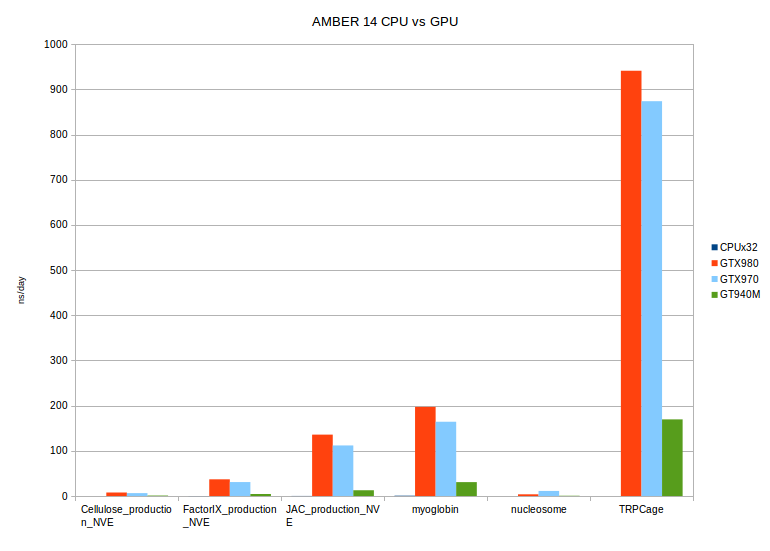
\includegraphics[width=1\textwidth]
	{pics/amber_mpi_cuda}
	\caption{Eksperimen AMBER pada GPU (CUDA) dan CPU \textit{cluster} (MPI)}
	\label{fig:amber_mpi_cuda}
\end{figure}  

Hasil yang kami dapatkan adalah direpresentasikan oleh diagram pada gambar \ref{fig:amber_mpi_cuda}. Pada hasil eksperimen ini kinerja (\textit{ns/day}) \textit{cluster} CPU (MPI) sangatlah kecil jika dibandingkan dengan kinerja semua tipe GPU, yaitu selalu di bawah 1,0. Nilai kinerja GPU yang tercepat adalah GTX 980 diikuti GTX 970 yang sedikit di bawahnya. Kinerja GPU 940M cukup jauh di bawah kedua GPU lainnya tapi tetap masih 2-30 kali lebih cepat daripada \textit{cluster CPU}.

Selain itu hasil eksperimen juga menunjukkan bahwa eksperimen dinamika molekular yang paling membutuhkan banyak sumber daya (\textit{ns/day} terkecil) adalah \verb|Cellulose Production NVE| dan \verb|Nucleosome Production| yang memiliki rasio jumlah atom : nsteps terbesar.

%-----------------------------------------------------------------------------%
\section{Kesimpulan}
%-----------------------------------------------------------------------------%

Berdasarkan hasil eksperimen yang kami lakukan, kami mengambil kesimpulan sebagai berikut:

\begin{enumerate}
	\item AMBER 14 berjalan jauh lebih efisien di GPU dibanding di CPU (MPI) bahkan sampai 200x lebih cepat (\verb|Myoglobin Production|) bahkan ketika dibandingkan dengan 940M yang termasuk kelas \textit{mainstream-mobile}.
	\item AMBER 14 menggunakan kemampuan GPU dengan optimal sehingga bias terlihat jelas perbedaan kemampuan antar GPU. Dalam eksperimen ini 940M yang merupakan GPU kelas \textit{mainstream-mobile} terlihat jelas kinerjanya jauh di bawah GTX 970 dan GTX 980 yang termasuk kelas \textit{high-end-PC}.
	\item Kebutuhan sumberdaya komputasi percobaan dinamika molekular tergantung pada banyaknya jumlah atom serta nsteps yang dilakukan. Semakin besar rasio jumlah atom : nsteps, maka semakin besar sumberdaya komputasi yang dibutuhkan dan semakin lama waktu proses yang dibutuhkan.
\end{enumerate}
